\documentclass[a4paper,12pt]{book}
\usepackage[utf8]{inputenc}

\usepackage{rachwidgets}


\newcommand{\laClass}       {CS 211}
\newcommand{\laSemester}    {Spring 2018}
\newcommand{\laChapter}     {5.4}
\newcommand{\laType}        {Exercise}
\newcommand{\laPoints}      {5}
\newcommand{\laTitle}       {Binary Sequences}
\newcommand{\laDate}        {Jan 25, 2018}
\setcounter{chapter}{5}
\setcounter{section}{4}
\addtocounter{section}{-1}
\newcounter{question}

\toggletrue{answerkey}
%\togglefalse{answerkey}


\title{}
\author{Rachel Singh}
\date{\today}

\pagestyle{fancy}
\fancyhf{}

\lhead{\laClass, \laSemester, \laDate}

\chead{}

\rhead{\laChapter\ \laType\ \iftoggle{answerkey}{ KEY }{}}

\rfoot{\thepage\ of \pageref{LastPage}}

\lfoot{\scriptsize By Rachel Singh, last updated \today}

\renewcommand{\headrulewidth}{2pt}
\renewcommand{\footrulewidth}{1pt}

\begin{document}




\footnotesize
~\\ 
\textbf{\laChapter\ \laType: } In-class exercises are meant to introduce you to a new topic
and provide some practice with the new topic. Work in a team of up to 4 people to complete this exercise.
You can work simultaneously on the problems, or work separate and then check your answers with each other.
Completion score is given for this assignment.

~\\
Team:\\
(1) \tab[6cm] (2) \\
(3) \tab[6cm] (4)

\hrulefill
\normalsize 


\notonkey{
% ASSIGNMENT ------------------------------------ %

    \section{\laTitle}
    
    \subsection{Binary sequences}

    \begin{intro}{Binary sequence theorem}
        \begin{quote}
			The number of binary sequences with $r$ 1's and $n-r$ 0's is $C(n,r)$ or $C(n, n-r)$.
			\footnote{From Discrete Mathematics, Ensley and Crawley, page 409}
        \end{quote}
        
        This can be used for straightforward problems, like ``how many binary sequences are there
        with $x$ 1's and $y$ 0's?'', but we can also use it for more practical applications...!
    \end{intro}

    \stepcounter{question}
    \begin{questionNOGRADE}{\thequestion}
        How many binary sequences are there with three 1's and two 0's?
        
        \begin{enumerate}
	        \item[a.]	How many 1's? $r = $
	        \item[b.]	How many 0's? $n-r = $
	        \item[c.]	What is the value of $n$?
	        \item[d.]	How many binary sequences are there? $C(n,r) = $
		\end{enumerate}
    \end{questionNOGRADE}
    
    \hrulefill
       
    \stepcounter{question}
    \begin{questionNOGRADE}{\thequestion}
	    Assuming you're building a binary string of length 5,
	    using the Binary Sequence theorem and the Sum Rule, 
	    find the number of binary sequences that have an odd number of 1's.
	    \\ \textit{(Hint: this means one 1, three 1's, or five 1's; you can figure out the 0's from that.)}
	\end{questionNOGRADE}
	
	\newpage
	
	\begin{intro}{Other uses of Binary Sequences}
		We can also use this theorem for strings that have more than just 0's and 1's...
		
		\paragraph{Example 2 from the book:} How many ordered lists of 10 letters, chosen from $\{m, a, t\}$, 
		have exactly three $m$'s?
		
		If we think in terms of spots to fill for each letter, we can diagram it like this:
		
		\begin{center}
			\begin{tabular}{c c c c c c c c c c}
				\fitb[0.5cm] & \fitb[0.5cm] & \fitb[0.5cm] & \fitb[0.5cm] & \fitb[0.5cm] & \fitb[0.5cm] & \fitb[0.5cm] & \fitb[0.5cm] & \fitb[0.5cm] & \fitb[0.5cm]
				\\
				1 & 2 & 3 & 4 & 5 & 6 & 7 & 8 & 9 & 10
			\end{tabular}
		\end{center}
		
		~\\ Since we have a restriction on the $m$'s, these should be filled in first. Selecting three $m$'s gives us
		$C(10,3) = 120$ combinations.
		
		~\\ Then, since there are no restrictions on the rest of the letters, we can select the final 7.
		However, we don't have 3 to choose from anymore; we wanted \textbf{exactly} 3 $m$'s and we have
		already filled those. So, instead of selecting from 3 options, we only have two: $\{a, t\}$.
		
		~\\ Since for each of the remaining, we have two options each, it will be calculated as $2 \cdot 2 \cdot 2 \cdot ...$
		seven times. These remaining 2's are an \textbf{ordered list}: Order matters, and we can have duplicates ($a$ or $t$).
		
		~\\ Our final result will be $C(10,3) \cdot 2^{7}$.
	\end{intro}
	
    \begin{intro}{Formulas for each structure type}
	
		\begin{center}
			\begin{tabular}{l | c | c | c }
				\textbf{}
					& \textbf{Repeats}
					& \textbf{Order}
					& \textbf{}
				\\
				\textbf{Type}
					& \textbf{allowed?}
					& \textbf{matters?}
					& \textbf{Formula}
				\\ \hline
				Ordered list of length $r$
					& yes
					& yes
					& $n^{r}$

				\\ \hline
				Unordered list of length $r$
					& yes
					& no
					& $C(r + n - 1, r)$
				\\ \hline
				Permutations of length $r$
					& no
					& yes
					& $P(n,r) = \frac{n!}{(n-r)!}$
				\\ \hline
				Sets of length $r$
					& no
					& no
					& $C(n,r) = \frac{n!}{r!(n-r)!}$
			\end{tabular}
		\end{center}
        
    \end{intro}

    We can also use what we've learned on application problems, where we need to
    group up items together.

    \newpage

    \begin{intro}{Modeling problems with binary sequences}
        Let's say you have a box that can store 8 donuts.
        If you're going to put multiple flavors in the box, you will
        use a separator to keep them apart.

        \begin{center}
            \begin{tabular}{c c}
                Same donuts & 
                Different donuts
                \\ \\
                \centering
                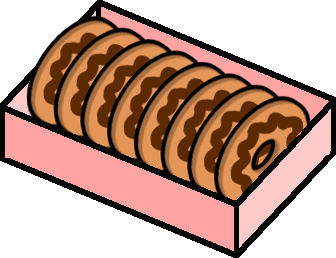
\includegraphics[width=6cm]{images/donutbox1.png}
                &
                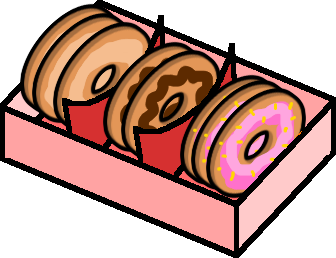
\includegraphics[width=6cm]{images/donutbox2.png}
            \end{tabular}
        \end{center}

        In this case, we don't care what kind of donuts are in the box;
        we will represent them with zeroes. The splitters, we will represent as 1.
        With this information, we will model our box of donuts as a binary string.

        \begin{center}
            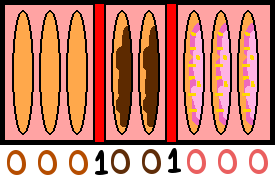
\includegraphics[height=4cm]{images/donutbox3.png}
        \end{center}
    \end{intro}
    
    \stepcounter{question}
    \begin{questionNOGRADE}{\thequestion}
        For the following donut combinations, draw the donut box, the donuts, and the separators.
        Also list out the binary sequence that represents the box.
        Assume that the box must always have 2 separators. If a separator isn't being used, it can
        go at either end of the box.

        \begin{enumerate}
            \item[a.]   One Chocolate, Three Strawberry, and Four Glazed
            \item[b.]   Four Chocolate and Four Glazed
            \item[c.]   Eight Glazed
        \end{enumerate}
    \end{questionNOGRADE}

    \newpage

    \begin{intro}{Theorem}
        Let natural numbers $n$ and $r$ be given.
        \footnote{Theorem 3 from Discrete Mathematics, Ensley and Crawley, page 413}

        \begin{enumerate}
            \item   The number of solutions to the equation $x_{1} + ... + x_{n} = r$
            using nonnegative integers is $C(r + n - 1, r)$.
            \item   The number of unordered lists of length $r$ taken from a set of size $n$,
            which repetitions allowed, is $C(r + n - 1, r)$.
            \item   The number of bags of $r$ pieces of fruit that can be bought at a store with $n$
            types of fruit available is $C(r + n - 1, r)$.
        \end{enumerate}
    \end{intro}
    
    \stepcounter{question}
    \begin{questionNOGRADE}{\thequestion}
        At Darrell's Donuts, Darrell sells 5 different types of donuts.
        He only sells 12-donut boxes. How many different combinations
        of donut boxes can you build?
        \footnote{Based on Example 6 from Discrete Mathematics, Ensley and Crawley, page 413}

        \begin{enumerate}
            \item[a.]   How many types of donuts are there? $n =$
            \item[b.]   How many donuts will be selected? $r = $
            \item[c.]   How many separators should there be?
                        \textit{(Hint: It should be one less than the donut types)}
            \item[d.]   If donuts and separators both count as spaces in the box,
                        how many available spaces are there total?
            \item[e.]   What is $r + n - 1$?
            \item[f.]   What is the Combination formula for finding out the total ways you can build your donut boxes?
            \item[g.]   What is the final answer?
        \end{enumerate}
    \end{questionNOGRADE}

    \hrulefill

    \stepcounter{question}
    \begin{questionNOGRADE}{\thequestion}
        At Piper's Produce, there are 3 types of fruit for sale.
        How many ways can you fill a bag that can store 20 pieces of fruit?
    \end{questionNOGRADE}
}{
% KEY ------------------------------------ %
    \begin{itemize}
		\item[1a.]	1x B, 3x A, 2x N.
		\item[1b.]	There are $C(6,1) = 6$ ways to place the B.
		\item[1c.]	There are $C(5,3) = 10$ ways to place the A's.
		\item[1d.]	There are $C(2,2) = 1$ ways to place the N's.
		\item[1e.]	Use the Rule of Products: $6 \cdot 10 \cdot 1 = 60$.
		
		\item[2.]	P: $C(12,1)$, E: $C(11,1)$, N: $C(10,3)$, S: $C(7,1)$, Y: $C(6,1)$, L: $C(5,1)$, V: $C(4,1)$, I: $C(3,1)$, A: $C(2,2)$ \\
					= $12 \cdot 11 \cdot 120 \cdot 7 \cdot 6 \cdot 5 \cdot 4 \cdot 3 \cdot 1$ \\
					= 39,916,800
                    
        \item[3a.]	$r = 3$
        \item[3b.]	$n-r = 2$
        \item[3c.]	$n-3 = 2$ \tab $n = 2 + 3$ \tab $n = 5$
        \item[3d.]	$C(n,r) = C(5,3) = 10$
        
        \item[4.]	Length 5 means 1x, 3x, or 5x ones.
					\\ one 1, four 0:	$r = 1$, $n-r = 4$, $n-1=4, n=5$, $C(5,1) = 5$
					\\ three 1, two 0:	$r = 3$, $n-r = 2$, $n-3=2, n=5$, $C(5,3) = 10$
					\\ five 1, zero 0:	$r = 5$, $n-r = 0$, $n-5=0, n=5$, $C(5,5) = 1$
					\\ $5 + 10 + 1 = 16$
		

        \item[5a.]  0100010000
        \item[5b.]  0000100001
        \item[5c.]  0000000011

        \item[6a.]  $n = 5$
        \item[6b.]  $r = 12$
        \item[6c.]  4 separators
        \item[6d.]  12 donuts + 4 separators = 16
        \item[6e.]  $r + n - 1 = 12 + 5 - 1 = 16$
        \item[6f.]  $C(16,12)$ or $C(16,4)$.
        \item[6g.]  $C(16,12) = 1,820$

        \item[7.]   20 pieces of fruit, 2 separators: $C(22,20)$. \\
                    $C(22,20) = 231$
    \end{itemize}
}



\end{document}

